%	JASA LaTeX Sample File, Preprint Sample
%
%  Beginner Latex users should refer to their favorite online documentation
%  here is one from the TeX Users Group 
%	https://www.tug.org/twg/mactex/tutorials/ltxprimer-1.0.pdf
%
%  Useful FAQ from  https://journals.aps.org/revtex/revtex-faq
% 




%%%%%%% For Preprint
%% For manuscript, 12pt, one column style

 \documentclass[preprint,NumberedRefs]{JASAnew}

%%%%% Preprint Options %%%%%
%% The track changes option allows you to mark changes
%% and will produce a list of changes, their line number
%% and page number at the end of the article.
%\documentclass[preprint,trackchanges]{JASAnew}

%% authaffil option will make affil immediately
% follow author, otherwise authors are grouped, and affiliations
% are stacked underneath all the authors.
%\documentclass[preprint,authaffil]{JASAnew}

%% NumberedRefs is used for numbered bibliography and citations.
%% Default is Author-Year style.
% \documentclass[preprint,NumberedRefs]{JASAnew}

%%%%%%% For Reprint
%% For appearance of finished article; 2 columns, 10 pt fonts

% \documentclass[reprint]{JASAnew}

%%%%% Reprint Options %%%%%

%% For testing to see if author has exceeded page length request, use 12pt option
% \documentclass[reprint,12pt]{JASAnew}

% authaffil option will make affil immediately
% follow author, otherwise authors are grouped, and affiliations
% are stacked underneath all the authors.
%\documentclass[reprint,authaffil]{JASAnew}

%% NumberedRefs is used for numbered bibliography and citations.
%% Default is Author-Year style.
% \documentclass[reprint,NumberedRefs]{JASAnew}

%% TurnOnLineNumbers
%% Make lines be numbered in reprint style:
% \documentclass[reprint,TurnOnLineNumbers]{JASAnew}

%%%Added by Aaron
%\usepackage{subcaption}

\begin{document}

\title[JASA Article]{Enhancing bowhead whale detection using convolutional autoencoders}
\author{Océane Boulais}

\affiliation{Marine Physical Laboratory, Scripps Institution of Oceanography,  University of California San Diego, La Jolla, CA 92093, USA}

\author{Aaron Thode}

\affiliation{Marine Physical Laboratory, Scripps Institution of Oceanography,  University of California San Diego, La Jolla, CA 92093, USA}

\author{Susanna B. Blackwell}
\affiliation{Greeneridge Sciences, Inc., 5266 Hollister Ave., Suite 107, Santa Barbara, California 93111, USA}

\preprint{Boulais 2026, JASA}		%  if you want want this message to appear in upper left corner of title page

\date{\today} 

\begin{abstract}
% Abstracts are limited to 200 words for
% regular articles. 

**Between 2007 and 2014, Greeneridge Sciences deployed 35 passive acoustic directional recorders along a 280 km swath of the Alaskan North Slope, funded by Shell Exploration and Production Company, to detect and localize bowhead whale calls during the annual fall migration.** Each season a team of manual analysts annotated the time, frequency range, distance, and type of bowhead calls, eventually labeling nearly 8.7 million call detections, one of the largest annotated bowhead whale sound datasets in existence. In 2010 a simple three-layer neural network was developed to localize millions of these calls, but it could only recognize, not classify, relatively simple frequency-modulated sounds**, at a natural false-positive-to-true-call ratio of roughly 8:1**. **Here we compare modern supervised and unsupervised deep learning methods for detecting these highly variable sounds.** A convolutional autoencoder compresses single-channel signal-to-noise-ratio spectrogram images into a 32-element feature vector. **A simple nearest-neighbor classifier built directly on this latent space, evaluated at a matched 10\% miss-fraction operating point, reduces the false-positive-to-true-call ratio to between 0.37:1 and 1.55:1 relative to each label set's own natural baseline (8.02:1 to 11.64:1), depending on the dataset label set and minimum call duration, and is our most readily reproducible detection result to date. The same encoder trunk separately backs a supervised convolutional classifier -- either randomly initialized or warm-started from the autoencoder and fine-tuned end-to-end -- to distinguish calls from other transients, including seismic airgun pulses. Both variants were trained on an identical, leakage-controlled 100,000-sample dataset and evaluated on an independent, 199,825-spectrogram held-out set spanning four field seasons (2008, 2010, 2012, 2014), generalizing similarly (ROC-AUC 0.959 vs.\ 0.956, average precision 0.805 vs.\ 0.787); unsupervised pretraining thus neither helped nor harmed detection performance here.**
\end{abstract}

%% pacs numbers not used

\maketitle

%  End of title page for Preprint option --------------------------------- %


\section{\label{sec:1} Introduction}

The Bering-Chukchi-Beaufort (BCB) population of bowhead whales is of great cultural importance to the Alaskan natives of the North Slope Borough. In the fall, the whales’ westward migration in the Beaufort Sea supports a subsistence hunt by three villages (Utqiaġvik, Nuiqsut, and Kaktovik), and by other villages in the Chukchi Sea.  The majority of the BCB population typically summers in the eastern Beaufort Sea (e.g., \cite{MooreReeves1993}). Beginning in late August, whales travel westward along the North Slope of Alaska, heading for their overwintering grounds in the Bering Sea. The fall migration in the Beaufort Sea is generally close and parallel to shore, mostly in water depths of 20–50 m \cite{WursigClark1993}.  
Passive acoustic monitoring provides an approach for monitoring the geographic distribution, seasonality, behavioral state, and potentially the relative abundance of bowhead whales\cite{szesciorka2024basin}. During the summer and fall, bowheads produce a variety of sounds which past work has roughly divided into “simple” frequency-modulated (FM) calls and “complex” calls\cite{ljungblad1982underwater, clark1986acoustic,clark1984sounds,cummings1987sounds, moore2006listening,blackwell2007bowhead,stafford2021acoustic}.  Simple calls (Figure 1) generally include up calls, down calls, inflected calls, and undulated calls \cite{WursigClark1993}, whereas complex calls (Figure 2) include high calls, pulsed tonal and pulsive calls\cite{clark1984sounds}. The original call classification that was developed in the 1980s and 1990s is still used today, and little new research has focused on distinguishing bowhead call types during the summer and fall \cite{thode2016source,thode2017decadal,blackwell2013effects,blackwell2015effects,thode2020roaring,thode2024statistical}.  



\begin{figure}
    \centering
    \includegraphics[width=1\linewidth]{Figures/Upsweep_examples.jpg}
    \caption{Examples of the diversity of frequency-modulated bowhead whale call “upsweeps”.  Each spectrogram duration is 3 seconds, showing 0-500 Hz bandwidth.  The last image on the lower right shows an example to two bowhead calls overlapping in time, but not in frequency.}
    \label{fig:Upsweep diversity}
\end{figure}
    
%The existence of multiple call types has been known for decades, but the function of different call types remains unknown and difficult to obtain.  Simple sounds may serve as contact calls; for example, Ref. [10] has described counter-calling in migrating bowheads using simple, individually distinctive calls, possibly to synchronize each other’s movements.  For complex calls, four different studies [11-13] have reported a preponderance of complex pulsive calls in active or sexually active groups of bowhead whales, but other studies [14, 15] were unable to find correlations between call types and behavior. 

% The sheer volume of raw passive acoustic data from arctic waters has motivated the development of methods for automatically detecting, classifying, and localizing bowhead sounds**ref check**. 

% ***Calls are challenging because of diversity and the presence of airguns**

The sheer volume of raw passive acoustic data from arctic waters, combined with the
need for timely analysis, has motivated the development of methods for automatically
detecting, classifying, and localizing bowhead sounds \cite{thode2012automated}. Such automated approaches have become increasingly
common across marine mammal monitoring more broadly, ranging from spectrogram-correlation
and pitch-tracking classifiers \cite{mellinger2000bowhead, baumgartner2011generalized}
to modern deep neural networks that can substantially lower false-alarm rates relative
to traditional detectors \cite{shiu2020deep, allen2021convolutional}.

However, bowhead calls are particularly challenging to detect automatically
for two reasons. First, the calls themselves are highly variable: even simple frequency-modulated sweeps so no stereotyped frequency range, duration, or spectral slope (Fig. \ref{fig:Upsweep diversity}. Furthermore, a substantial fraction of sounds are not simple frequency-modulated moans and are typically lumped into a generic "complex" category
\cite{clark1984sounds, stafford2021acoustic} that incorporates sounds variously described as growls or grunts. The second challenge to automated classification is that during the fall migration the calls
can co-occur with seismic airgun pulses that overlap the same low-frequency band
(below 500 Hz), masking true calls and generating frequency-modulated transient signals that display similar bandwidth and time-frequency structure as bowhead calls\cite{blackwell2015effects, thode2012automated}.
%In this chapter we mine a unique long-term acoustic dataset to determine whether modern unsupervised deep learning machine learning techniques can be used to improve the detection and classification of bowhead whales sounds during their fall migrations.  

A previous automated detector and localizer has previously been developed by one of the PIs, that could detect specific call types but not classify them \cite{thode2012automated}.  This original algorithm used image processing to create hand-crafted feature vectors that were then passed through a simple three-layer neural network to flag whether a sound was a whale call or not.  This algorithm could thus be used to compute call rates and call spatial densities and has been applied to multiple previous studies\cite{thode2016source,thode2017decadal,thode2020roaring,thode2024statistical,blackwell2015effects}.  


Here we apply modern supervised convolutional neural networks (CNN) and unsupervised convolutional autoencoders\cite{guo2017deep,ozanich2021deep} to extract latent feature vectors directly from spectrogram images, without human design and input.


%We then evaluate whether initializing a supervised call and non-call classifier from this unsupervised representation (rather than training the same classifier architecture from random weights) measurably improves detection performance.

Section II describes the equipment, deployment geometry, and data preprocessing used to create both training and evaluation datasets.  It then describes the convolutional autoencoder architecture used to process the data, the supervised classifier built on top of it, and the training and evaluation procedures used to compare the two initialization strategies.  Section III reports the resulting detection performance using the evaluation datasets, and highlights the importance of identifying and removing data samples that contain multiple sources, such as two whale calls, or a whale call and an airgun.  It also discusses the utility of using dimensionality reduction and visualization methods on the latent feature space to correct and re-label mis-classified data. 

%evaluated on a held-out set that is fully independent of the training data.

The paper is organized as follows: Section~\ref{sec:Methods} presents
information about the acoustic dataset, the autoencoder and classifier architectures,
and the training/evaluation protocol. Section~\ref{sec:Results} reports the detection
performance of the two classifier initialization strategies on the independent
held-out evaluation set. Section~\ref{sec:Conclusion} discusses the implications of
these results and outstanding questions for future work.


\section{\label{sec:Methods} Methods}

\subsection{\label{sec:DataOverview}Acoustic Data}

\begin{figure}
    \centering
    \includegraphics[width=1\linewidth]{Figures/DASAR_map.jpg}
    \caption{:  Locations of the five DASAR sites (arrays, sites 1-5) in the Beaufort Sea, 2007–2014.  The inset shows the location of the map on the north coast of Alaska.  After 2011 Site 4 “flipped” four DASAR locations from the blue triangles to the hollow orange triangles.  This chapter uses data from Sites 3 and 5.}
    \label{fig:DASAR_map}
\end{figure}
Between 2007 and 2014, as part of their exploration activities in the Beaufort Sea, the Shell Exploration and Production Company implemented an acoustic monitoring program to study the effects of industrial activities, particularly seismic airgun surveys, on bowhead whales during their fall migration (August–October). Arrays of Directional Autonomous Seafloor Acoustic Recorders (DASARs)\citep{greene2004directional} were deployed at five sites in the Beaufort Sea between Kaktovik and Harrison Bay, a 280 km span (Fig. 3)\cite{blackwell2015effects}.  
 

DASARs are autonomous recording packages equipped with an DIFAR sonobuoy vector sensor package\cite{holler2014evolution,Kuzu6459697_DIFAR}, consisting of a omnidirectional acoustic pressure sensor (sensitivity of 149 dB re 1 $\mu$Pa/V) and two horizontal directional sensors capable of measuring the north-south and east-west components of acoustic particle velocity\cite{greene2004directional}.  This arrangement permits the azimuth of received sounds, such as bowhead whale calls, to be measured from individual DASARs.  Each time series is sampled at 1 kHz with a maximum usable acoustic frequency of 450 Hz due to antialiasing filter roll-off.  
Each site consisted of three to 11 DASARs deployed in a triangular grid with 7 km separation; individual instruments are labeled ‘A’ through ‘G’ from south to north (Fig. 3).  Within a site, a unique call is often detected across multiple DASARS, and the resulting bearings can be triangulated to measure a whale’s location.  To avoid confusion, we define a “unique call” (UC) as a sound generated by a whale at a specific time and location, while a “call detection” (CD) is defined as the signal detected by a specific DASAR resulting from that unique call.  Thus, multiple CDs can result from a single UC, and by triangulating the bearings from the set of CDs (“CD set”) the generation time and location of the original UC can be estimated.  As a byproduct the tracking system records samples of the same UC at multiple ranges; however, the positions and ranges of calls are not used in the deep learning analysis presented here.

\subsection{Initial Manual Analysis}

A subset of data from all years (typically 5 – 8 days) was also processed manually. Over the span of eight years, 8,690,929 CDs were reviewed by experienced manual analysts with multiple years of experience.  The analysts measured each CD's frequency span, duration, and bearing.  They then assigned sets of CDs to the same UC, localized the UC, and then classified the UC into various types of simple and complex calls, including up calls, down calls, undulations, tonal (constant frequency), and “complex calls”, a catch-all category that spans various kinds of calls that cannot be assigned to another category.  This combined manual and automated database remains one of the largest compiled datasets of bowhead sounds in existence and may represent the largest annotated dataset of localized bowhead call types in the world.

\subsection{Dataset construction}
\subsubsection{Data subsets}
Training sets for the deep learning algorithm were set to 100,000 samples, which were selected from Sites 3 and 5 during the years 2008, 2010, 2012, and 2014 (a total of 24 date/DASAR combinations).  DASARS ‘A’,’D’, and ‘G’, which represent the shallowest, median, and deepest water depths, were used from each site.   This subselection ensured that the deep learning algorithms would be trained on data that covered a variety of water depths between 30 and 55 m.   Sampling data across years permitted us to cover the full time span for the training set, an important consideration as evidence exists that the frequency content of the bowhead calls evolved across the years of the experiment\cite{thode2017decadal}.  

For each year 5-8 days were sampled, corresponding to dates when manual analysis was also conducted.  For a given year, all DASARs at all sites were sampled on the same day, but the dates sampled varied between years, as the DASARs were deployed on slightly different dates each year.  Any difference between days sampled at Sites 3 and 5 for a given year arose because the sites were deployed and recovered at slightly different dates at the start and end of that year’s deployment.  The number of samples for a given year/DASAR combination in the training dataset was proportional to the fraction of signals present for that year/DASAR combination in the entire manually-analyzed dataset.  Thus the training dataset reflected the time and space distribution of whale calls through the entire dataset.  Table I lists the dates used for every site/year combination.  

\begin{table}[ht]
    \centering
    \caption{Dates used for training dataset as a function of year and site.}
    \label{tab:training_dates}
    \begin{tabular}{|c | c | c|}
        \hline
        Year & Site 3 & Site 5 \\
        \hline
        2008 & 8/28, 9/06, 9/13, 9/21, 9/29 & Same but also 8/21 \\
        2010 & 8/15, 8/21, 8/29, 9/05, 9/13, 9/27 & Same but no 9/27 \\
        2012 & 8/25, 9/01, 9/07, 9/13, 9/18, 9/23, 9/29, 10/05 & Same but no 9/07 or 10/05 \\
        2014 & 8/18, 8/28, 9/01, 9/17, 9/27 & Same \\
        \hline
    \end{tabular}
\end{table}

\subsubsection{\label{sec:EventDetection}Transient Detector}

To convert the raw acoustic data streams into discrete call samples to be fed into an autoencoder, a simple transient detector was applied to DASARs A,D, and G over the full 24-hour dataset for each day listed in Table \ref{tab:training_dates}.  No information from the manual database was applied during this initial event detection stage, to ensure that whale calls would be treated consistently with all other transient signals.

The transient detector was an “energy” constant false alarm rate (CFAR) transient detector originally developed for the original detection algorithm\cite{thode2012automated}.  The detector used at 256-point Fast Fourier Transform (FFT) with 75\% overlap to compute a moving average of the background noise spectrum to which a new incoming spectrum was compared.  The time constant (equalization time) of the moving average was 25 seconds, and the spectrogram was converted to units of power spectral density (dB re 1 $\mu Pa^2$/Hz).   A filter bank of detectors was created, each covering 40 Hz in bandwidth, overlapped 50\%.  The lowest frequency detector thus spanned 25 to 65 Hz, the second band 45 to 85 Hz, and so on up to 450 Hz.  

The purpose of running a filterbank of detectors was to avoid missing signals that were locally narrowband but high signal-to-noise ratio (SNR).  Other transient detectors have also been proposed for enhancing detection of locally narrowband signals across a wide frequency span \cite{wang2001all, helble2012generalized}.
The start of a new detection was logged whenever the integrated spectrum of any detection band in a new incoming FFT exceeded 5 dB SNR relative to the corresponding background noise band, and that threshold endured for at least 100 msec.  The detection was logged as ending when all detection bands fell below the 5 dB threshold.  Detections logged less than 50 msec from the previous detection were merged with the previous detection.

\subsubsection{Training and Evaluation Datasets}
\label{sec:Training Dataset Construction}
Next, each transient detection was compared against the manual database to see whether the transient's time window overlapped a manual annotation time window by 50\% or more, ignoring annotations flagged as seals or unknown biologics.  If this overlap threshold was exceeded, the transient was flagged as an 'annotation' and assigned the classification label associated with the annotation.  If a transient was sufficiently long to encompass multiple annotations, the earliest annotation was used.  **[TODO: fill in the percentage of manual annotations that did not overlap any transient detection; not yet computed in this pass]**

For every transient (regardless of whether it is matched with an annotated whale call), five seconds of acoustic data were extracted from the omnidirectional channel, centered around the time of maximum peak power encountered across any filterbank.  A new spectrogram was created with a 256 pt FFT (90\% overlap) and converted to units of power spectral density (dB re 1 $\mu Pa^2$/Hz).  The median background spectrum was estimated from samples present in the first and last seconds of the time window and then subtracted from the middle three seconds of the spectrogram, to convert the image into units of dB SNR.  The final spectrogram image was 128 frequency bins by 119 time bins, spanning a fixed time window of three seconds and a bandwidth of 25 to 500 Hz.  An point crucial to future discussion is that the images were centered around the time of peak local power spectral density encountered between 25 and 450 Hz, to reduce the tendency of the autoencoder to map time-shifted signals into different parts of the feature space.  The images were stored as unsigned 8-bit integer resolution to make efficient use of memory.

The total number of transients extracted from all the dates in Table \ref{tab:training_dates} was 2,116,248, of which 238,751 were annotations, a ratio of 7.86 unmatched transients per manual annotation.  However, the ratio of transients to annotations, computed over one day, varied by date and Site.

From this master database we constructed both a 100,000 sample 'training' dataset and a 200,000 sample 'evaluation' dataset.  For the training dataset, we randomly selected 46,549 annotations and 53,451 transients (not associated with a manual annotation) without replacement from the master database, to create a more balanced dataset with greater representation of whale calls.  Both annotations and transients were sampled in proportion to their total distribution across year, day, and Site, so that the random subsample accurately represented the characteristics of the full database.

The evaluation dataset consisted of 199,825 transients and 22,181 annotations, to reflect the true expected ratio of transients to annotations in the full dataset.  It was important to do this because evaluation metrics like 'precision' are affected by the number of true negatives in the dataset.

A substantial number of transient detections were seismic airgun signals (20365 out of 50000, or 40.4 \%).

The supervised classifier described in Sec.~\ref{sec:cnn_classifier} was trained on a
separate, matched 100,000-sample draw from the same pool of transient detections (50,000
manually-verified calls, Types 1--7, and 50,000 auto-detected non-call transients, Type 0,
subsampled without replacement using a fixed random seed), so that the scratch- and
warm-start-initialized classifiers could be compared on identical training data. This
draw spanned only DASAR sites 3 and 5 (site 3: 50,503 images; site 5: 49,497 images) and
DASARs A, D, and G (36,311; 36,298; and 27,391 images respectively), with call sub-type
counts of 14,693 (Type 1), 10,750 (Type 2), 7,968 (Type 3), 4,763 (Type 4), 3,457 (Type
5), 1,553 (Type 6), and 6,816 (Type 7).


 

\subsection{\label{sec:autoencoder}Autoencoder architecture, training, and dimension reduction}

% \begin{figure}
%     \centering
%     \includegraphics[width=0.75\linewidth]{Figures/Convolutional_Autoencoder_architecture.jpg}
%     \caption{Architecture of convolutional autoencoder}
%     \label{fig:autoencoder architecture}
% \end{figure}

% \begin{figure}[htbp]
%     \centering
%     \includegraphics[width=1\textwidth]{Figures/LD32_Updated_AE_Architecture.png}
%     \caption{Hybrid convolutional autoencoder architecture for bowhead whale call 
%     representation learning. The encoder accepts a 2-channel input: a spectrogram of the signal to noise ratio (\texttt{SNR\_gram}) and the normalised transport velocity (\texttt{NTV\_gram}), each $121\times104$ pixels, and 
%     applies three successive \texttt{Conv2d}+BatchNorm+ReLU+MaxPool blocks 
%     ($32{\to}64{\to}128$ channels), progressively halving spatial resolution while 
%     deepening feature representations. The resulting feature volume is flattened and 
%     passed through two fully connected layers (\textsc{fc}\,64, \textsc{fc}\,32) to 
%     produce a 32-dimensional latent embedding $\mathbf{z} \in \mathbb{R}^{32}$. The 
%     decoder mirrors this process: two fully connected layers (\textsc{fc}\,64) 
%     expand the latent code, a reshape operation restores spatial structure 
%     (128 channels, 13 rows), and three transposed convolution blocks reconstruct 
%     the original spatial dimensions, yielding a 2-channel output matching the input. 
%     Training minimises mean squared reconstruction loss across both channels 
%     simultaneously.}
%     \label{fig:autoencoder_architecture}
% \end{figure}


\begin{figure}[htbp]
    \centering
    \includegraphics[width=1.1\textwidth]{Figures/autoencoder_arch_Autoencoder_v13_100E_32LD_32C_AutoManual_Combined_100K_Date20260416-180022.png}
    \caption{Convolutional autoencoder architecture for bowhead whale call representation. The encoder reduces a single-channel spectrogram ($1\times121\times104$; 0–500 Hz, 3 s) through three Conv2D(3$\times$3)+BatchNorm+ReLU+MaxPool2D(2$\times$2) blocks, doubling channel depth at each stage ($32\to64\to128$) while halving spatial resolution to $128\times15\times13$. The flattened feature map (24,960 elements) is projected to a 32-dimensional latent vector via two FC layers (24960$\to$64$\to$32). The decoder mirrors this path (32$\to$64$\to$24960, reshape to $128\times15\times13$) and reconstructs the original dimensions through three ConvTranspose2D(2$\times$2, stride=2)+BatchNorm+ReLU blocks, with output padding (1,0) on the final layer to recover the asymmetric input shape. Total trainable parameters: 3,358,593. Trained with Adam (lr=0.001), MSE loss, 100 epochs, 100K spectrogram samples.}
    \label{fig:autoencoder_architecture}
\end{figure}

The unsupervised deep learning architecture used for this study was a convolutional autoencoder \cite{hinton2006reducing}, which has been successful in the past for compressing acoustic signals \cite{ozanich2021deep,chien2023automatic}. We built the system in the open-source framework PyTorch \cite{paszke2019pytorch}, which began by normalizing each training spectrogram image (121 frequency bins $\times$ 104 time bins) so its pixel values ranged from 0 to 1 using min-max normalization applied independently to each sample. The image was then passed through three successive convolutional blocks, each consisting of a 3$\times$3 convolutional kernel with stride one and same-padding (padding=1), followed by batch normalization \cite{ioffe2015batch}, a ReLU activation \cite{nair2010rectified}, and 2$\times$2 max pooling \cite{lecun1998gradient}. The number of feature channels increased from 32 to 64 to 128 across the three blocks, while max pooling halved both spatial dimensions at each step, reducing the 121$\times$104 input to 15$\times$13 feature maps after the third block. The resulting 128-channel feature maps were flattened to a 24,960-element vector (128 $\times$ 15 $\times$ 13) and passed through two fully connected layers (24,960$\to$64$\to$32) with a ReLU activation between them, producing a 32-dimensional latent vector. The decoder first expands this latent vector back through two fully connected layers (32$\to$64$\to$24,960) with ReLU, reshapes the result to 128$\times$15$\times$13, and then applies three transposed convolutional layers (2$\times$2 kernel, stride 2) that progressively expand the feature maps from 128 to 64 to 32 channels — the first two blocks followed by batch normalization and ReLU — before a final transposed convolution projects back to a single-channel output at the original 121$\times$104 resolution. The decoder output is not passed through a sigmoid or clamping function, leaving the reconstruction unconstrained in value. Training was performed using the Adam optimizer \cite{kingma2015adam} (learning rate of $10^-3$) to minimize pixel-wise mean squared error (MSE) between the input and reconstructed spectrogram. Figure \ref{fig:autoencoder_architecture} illustrates the full encoder–decoder structure.

The system was trained for 100 epochs on the training dataset with a mini-batch size of 32. Reconstructed images were spot-checked against original images to qualitatively verify that the latent space had sufficient dimensions to reproduce the original signals (Fig.~\ref{fig:Reconstruction_Example}). Through this approach we determined that 16 dimensions were insufficient for representing the full repertoire of whale calls. 

To use the AE latent space as a detector, a nearest-neighbor algorithm (Euclidean distance) was used to compare a given evaluation sample against the samples in the training dataset.  The fraction of training neighbors that were annotated was then compared against a threshold to determine whether the evaluation sample would be classified as a whale call.  By adjusting the threshold a complete precision/recall curve could be generated.

\subsection{Supervised CNN classifier}
\label{sec:cnn_classifier}

To complement the unsupervised autoencoder, a supervised convolutional binary detector was built by attaching a linear softmax head directly to the
autoencoder's encoder trunk (three Conv+BatchNorm+ReLU+MaxPool blocks
followed by the FC-64$\to$FC-32 bottleneck; Fig.~\ref{fig:autoencoder_architecture}),
trained end-to-end with class-weighted cross-entropy. Annotated samples were labeled as whale calls, while non-annotated samples were treated as non-whale calls.  Two training regimes
were compared to isolate the contribution of the unsupervised pretraining:

\begin{itemize}
    \item \textbf{Scratch}: the encoder trunk is randomly initialized and
    trained jointly with the classification head.
    \item \textbf{Warm-start}: the encoder trunk is initialized from the trained autoencoder's weights (Sec.~\ref{sec:autoencoder}) and then
    fine-tuned jointly with the classification head. Of the encoder's 27 weight tensors, 25 were successfully transferred from the autoencoder checkpoint; the remaining 2 (belonging to the newly-added classification head) were randomly initialized, since the autoencoder has no
    equivalent layer.
\end{itemize}

Both variants were trained with the Adam optimiser (learning rate
$10^{-3}$, batch size 32), with early stopping after 10 epochs without
improvement in validation ROC-AUC (a ceiling of 100 epochs was never
approached: both runs stopped at epoch 12, with the best validation
ROC-AUC obtained at epoch 2 in both cases — 0.9533 for the scratch model
and 0.9469 for the warm-start model — after which validation ROC-AUC
declined monotonically while training loss continued to fall, indicating
overfitting to the training partition beyond this point).

\subsubsection{Leakage-free evaluation splits}
Because a single unique call (UC) is frequently detected redundantly across
multiple DASARs (A/D/G) on the same recording day, a naive random
per-image train/test split would place near-duplicate views of the same
call on both sides of the split, inflating performance metrics. All
train/validation/test splits were therefore constructed using a
\emph{grouped}, stratified partitioning scheme, with the group key set to
the date$\times$site combination (51 distinct date$\times$site groups
across the full 100,000-image training draw): every image recorded at a
given site on a given day was assigned entirely to one partition (train,
validation, or test), and the partitions were verified computationally to
share zero group overlap. Models were trained on a nominal 70/15/15
train/validation/test split (realised here as 70,870 training images
across 36 groups, 12,746 validation images across 7 groups, and 16,384
test images across 8 groups, each partition retaining an approximately
balanced call fraction of 0.49--0.53), with the validation split used only
for early-stopping model selection.

\subsubsection{Realistic-prevalence evaluation}
The training dataset used a class-balanced (approximately 1:1 annotated:transient) sample ratio
to stabilise optimisation. Because the deployment prevalence of whale calls in the true database is
substantially lower (approximately 1 call per 8 non-call transients, as
determined from Sec.~\ref{sec:Training Dataset Construction}), all reported test-set
average-precision values were computed after resampling the held-out test
set's negative class to match this $\approx$1:9 realistic prevalence,
while ROC-AUC (a prevalence-invariant metric) was computed on the full
held-out set as-is.

\subsubsection{Held-out evaluation dataset}
Both classifiers were subsequently scored, without any further training or
fine-tuning, against the independent held-out evaluation dataset discussed previously in Section \ref{sec:Training Dataset Construction}.

%consisting of 199,825 spectrograms spanning DASAR sites 3 and 5 and years 2008, 2010, 2012, and 2014 (22,159 manually verified bowhead calls, Types 1--7; 177,666 auto-detected non-call transients, Type 0; natural prevalence 0.1109). This evaluation directory is entirely disjoint from the 100,000 training images used inSec.~\ref{sec:cnn_classifier}:

The evaluation dataset was compiled and
stored separately, and no image, date, site, or DASAR combination present
in the training draw was reused as evaluation data. This constitutes a
substantially stricter generalisation test than the internal held-out test
split described above, since the internal test split — while
group-disjoint from the training set — is still drawn from the same
underlying collection process and the same restricted set of sites,
DASARs, and sampled dates as the training data, whereas the independent
evaluation directory was compiled, labeled, and stored as an entirely
separate artifact.


\subsection{Dimensionality reduction, visualization, and final manual review}
\label{sec:DatasetEditing}
To visualize the resulting latent space, the 32-dimensional latent representations were reduced to three dimensions using the Uniform Manifold Approximation and Projection (UMAP) algorithm \cite{mcinnes2018umap} with 15 nearest neighbors and a minimum distance of 0.1.  A special graphical user interface (GUI) was written in the programming language MATLAB that permitted an analyst to display and rotate the three-dimensional latent space UMAP representation, and then color the samples according to whether they had been annotated whale calls or other transients (Section \ref{sec:Training Dataset Construction}).  A user could select a subset of samples and review their associated input images.  

This ability to visualize the latent space proved extremely helpful in identifying mislabeled data from the original manual analysis.  The initial results of the autoencoder training indicated that some transients were legitimate whale calls (calls missed by the initial manual review), while some annotations were not whale calls (signals misidentified as whale calls), primarily arising from airgun signals masking a true call.  A significant number of samples were also found to contain multiple signals in the image window, such as a whale call and an airgun signal, or multiple overlapping whale calls.  The presence of multiple signals degraded automated performance significantly.  

We thus modified the visualization GUI to permit users to review and re-label samples as either whale calls, non-whale signals, or as multiple signals. Both the original annotations and the revised annotations were stored with the datasets and used to evaluate to what extent misclassified data impacts the supervised CNN and unsupervised AE.

\begin{figure}[htbp]
    \centering
    \includegraphics[width=1.1\textwidth]
    {Figures/reconstructions_Autoencoder_v13_100E_32LD_32C_AutoManual_Combined_100K_Date20260416-180022.png}
    \caption{Comparison between original input images (top) and the autoencoder's reconstructed (bottom) images from 32-dimension latent space of the 3 second recordings with time on the x-axis and frequency in Hz on the y-axis.}
    \label{fig:Reconstruction_Example}
\end{figure}



\section{\label{sec:Results} Results}

\subsection{Internal held-out test performance}

\begin{table}[ht]
    \centering
    \caption{Held-out \emph{internal} test performance of the supervised CNN detector
    (i.e., evaluated on the 15\% grouped test split carved from the same
    100,000-image training draw described in Sec.~\ref{sec:cnn_classifier}),
    comparing random initialization against warm-starting the encoder trunk from the
    convolutional autoencoder. Metrics are reported at the realistic
    $\approx$1:9 call:transient prevalence (Sec.~\ref{sec:cnn_classifier}).}
    \label{tab:cnn_results}
    \begin{tabular}{|l|c|c|c|c|}
        \hline
        Model & Test $N$ & ROC-AUC & Avg.\ Precision & Precision @ Recall=0.70 \\
        \hline
        Scratch (random init)     & 16{,}384 & 0.968 & 0.840 & 0.842 \\
        Warm-start (AE-init)      & 16{,}384 & 0.964 & 0.825 & 0.810 \\
        \hline
    \end{tabular}
\end{table}

% \begin{figure}[htbp]
%     \centering
%     \includegraphics[width=0.75\textwidth]
%     {Figures/poc_internal.png}
%     \caption{}
%     \label{fig:Internal POC}
% \end{figure}

% \begin{figure}[htbp]
%     \centering
%     \includegraphics[width=0.75\textwidth]
%     {Figures/fdr_internal.png}
%     \caption{}
%     \label{fig:Internal FDR vs Missed Fraction}
% \end{figure}


\subsection{Independent held-out evaluation performance}

\begin{table}[ht]
    \centering
    \caption{**Detection** performance of the two classifier initialization strategies on
    the fully independent 199,825-spectrogram held-out evaluation directory
    described in Sec.~\ref{sec:cnn_classifier} (natural prevalence 0.1109; both
    models scored without any further training on this data). This is the primary
    measure of real-world generalisation, since — unlike the internal test split of
    Table~\ref{tab:cnn_results} — this evaluation directory was compiled and stored
    entirely independently of the training data.}
    \label{tab:benchmark_results}
    \begin{tabular}{|l|c|c|c|c|}
        \hline
        Model & Embedding dim. & ROC-AUC & Avg.\ Precision & Precision @ Recall=0.70 \\
        \hline
        Custom CNN (scratch)      & 32   & 0.959 & 0.805 & 0.767 \\
        Custom CNN (warm-start)   & 32   & 0.956 & 0.787 & 0.741 \\
        \hline
    \end{tabular}
\end{table}

\begin{figure}[htbp]
    \centering
    \includegraphics[width=1.1\textwidth]
    {Figures/fdr_roc_external.png}
    \caption{Left side figure plots the precision–recall curves for bowhead whale call detection on the held-out evaluation set (n=199,825, prevalence=0.111), comparing random-initialization (scratch CNN: ROC-AUC=0.959, AP=0.805) versus warm-start initialization from a 32-dimensional convolutional autoencoder (ROC-AUC=0.956, AP=0.787). 
    % The minimal performance gap (~0.003 in ROC-AUC, ~0.018 in average precision) indicates that unsupervised pretraining provides no measurable generalization advantage over supervised training from random weights on this leakage-free dataset. 
    The right side figure plots false discovery rate (FDR) versus missed-detection fraction on the held-out evaluation set (n=199,825 spectrograms, realistic prevalence=0.111). Both the scratch-initialized CNN (blue) and warm-start CNN initialized from autoencoder weights (orange) achieve similar operating characteristics across the decision-threshold trade-off space, with the scratch-initialized CNN model slightly favoring lower false-discovery rates at high-recall operating points.}
    \label{fig: External FDR-ROC}
\end{figure}

% \begin{figure}[htbp]
%     \centering
%     \includegraphics[width=0.75\textwidth]
%     {Figures/external_precision_recall_curve.png}
%     \caption{}
%     \label{fig:External POC}
% \end{figure}

On this independent evaluation set, both classifiers generalise to essentially the
same degree: the scratch-initialised model outperforms the warm-start model by a
narrow, likely practically-insignificant margin on every metric (0.003 in ROC-AUC,
0.018 in average precision, 0.026 in precision at fixed recall). Performance was
also consistent across evaluation subgroups: broken down by year, ROC-AUC ranged from
0.951--0.961 (scratch) and 0.951--0.956 (warm-start) across the four field seasons
(2008, 2010, 2012, 2014); broken down by site, ROC-AUC ranged from 0.954--0.964
(scratch) and 0.952--0.960 (warm-start) across sites 3 and 5; and broken down by
DASAR, ROC-AUC ranged from 0.957--0.963 (scratch) and 0.953--0.959 (warm-start)
across DASARs A, D, and G. The absence of any subgroup in which either model
collapses toward chance-level performance (ROC-AUC $\approx$ 0.5) indicates that
this small scratch-vs-warm-start gap is a stable, genuine property of the two
initialization strategies on this dataset, rather than an artifact confined to a
particular year, site, or recording condition. We note that unsupervised
autoencoder pretraining is therefore not shown here to confer a measurable
generalisation advantage over training the same classifier architecture from
random initialization; whether this null result reflects a genuine property of
this task and dataset, or a limitation of the specific autoencoder pretraining
recipe used here (e.g., its purely reconstructive, non-contrastive objective, or
the modest scale of the 32-dimensional latent bottleneck), is discussed further
in Sec.~\ref{sec:Conclusion}.

\subsection{Effect of dataset relabeling on CNN detection performance}
\label{sec:CNNRelabel}

The dataset-editing pass described in Sec.~\ref{sec:DatasetEditing} raises a
natural question: how much of the scratch CNN's detection performance
(Table~\ref{tab:benchmark_results}) is attributable to the classifier itself,
versus the quality of the labels it is scored against? To isolate this, the
same frozen scratch-CNN checkpoint used in Table~\ref{tab:benchmark_results}
was scored exactly once on the 199,825-spectrogram independent evaluation
set, producing a single, fixed set of call probabilities; these same
probabilities were then re-graded against two label sets pulled from the
same underlying MATLAB export: the \emph{original}, pre-review labels
(\texttt{type\_org}) and the manually \emph{reviewed} labels (\texttt{iscall})
produced by the latent-space-guided relabeling pass of
Sec.~\ref{sec:DatasetEditing}. Because the model's outputs are identical in
both cases, any difference in reported performance isolates the effect of
correcting mislabeled evaluation examples from any change in the detector
itself. In total, 6,345 of the 199,825 labels (3.2\%) were changed by the
review, most often airgun pulses previously mislabeled as calls, or calls
missed by the original manual pass.

\begin{table}[ht]
    \centering
    \caption{Scratch CNN detection performance on the 199,825-spectrogram
    independent evaluation set, scored once and re-graded against the
    original (pre-review) vs.\ manually reviewed (post-review) label sets, at
    a matched operating point of miss fraction = 10\% (recall = 0.90) for both
    label sets, so the two rows are compared at an equal fraction of true
    calls found rather than at two different, unmatched recall levels.
    ``Prevalence'' is the fraction of the 199,825 evaluation spectrograms
    labeled a call under that label set; ``FDR'' (false discovery rate,
    $1-$precision) is the fraction of samples flagged as calls, at this
    10\%-miss operating point, that are not actually calls.
    6,345 of 199,825 labels (3.2\%) differ between the two label sets.}
    \label{tab:cnn_relabel_results}
    \begin{tabular}{|l|c|c|c|c|}
        \hline
        Label set & Prevalence & ROC-AUC & Miss fraction & FDR \\
        \hline
        Original (pre-review)  & 0.1109 & 0.964 & 10.0\% & 0.448 \\
        Reviewed (post-review) & 0.0791 & 0.980 & 10.0\% & 0.405 \\
        \hline
    \end{tabular}
\end{table}

\begin{figure}[htbp]
    \centering
    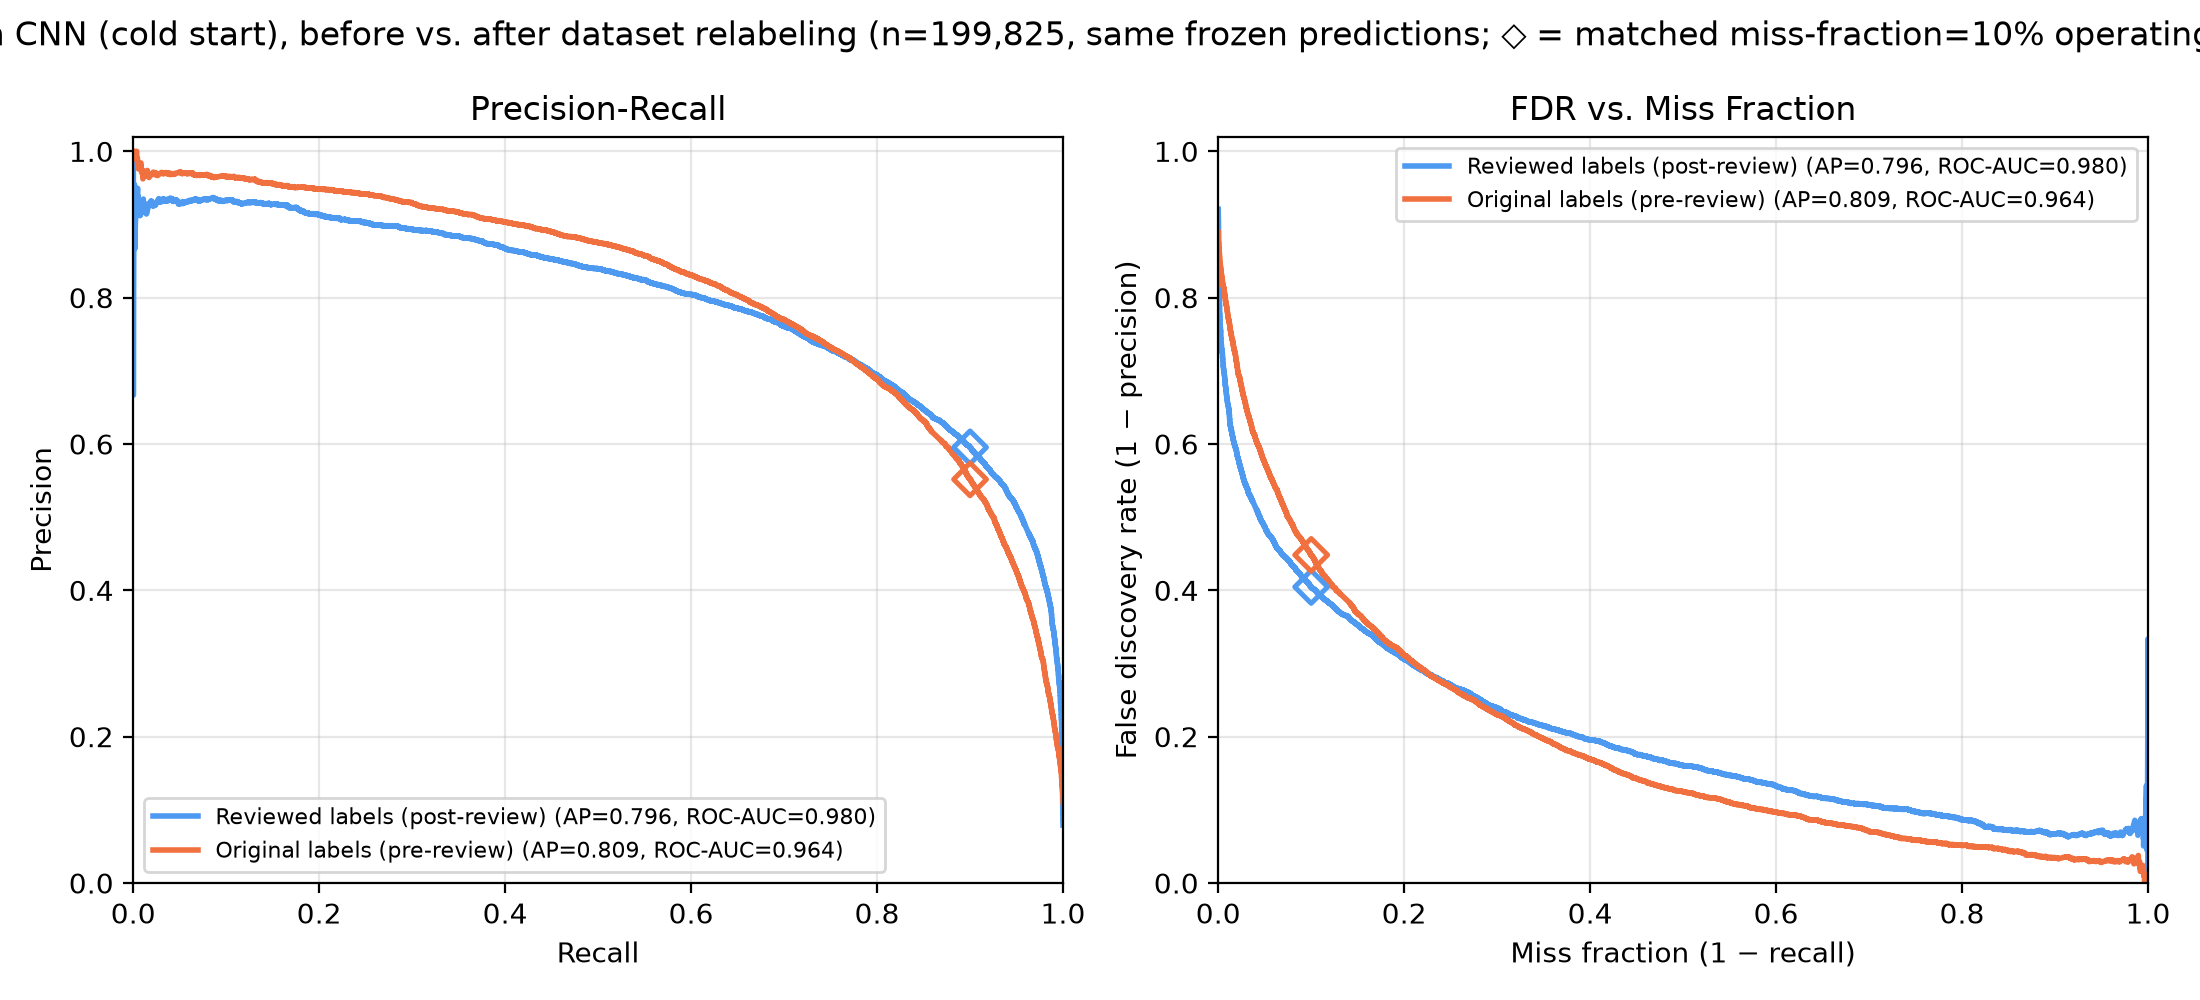
\includegraphics[width=1.1\textwidth]{Figures/cnn_relabel_pr_fdr.png}
    \caption{Left: precision--recall curves for the same frozen scratch-CNN
    predictions on the 199,825-spectrogram independent evaluation set, scored
    against the original pre-review labels (orange, AP=0.809) versus the
    manually reviewed post-review labels (blue, AP=0.796). Right: the same
    comparison expressed as false discovery rate vs.\ miss fraction. Diamond
    markers on both panels mark the matched miss-fraction=10\% operating
    point reported in Table~\ref{tab:cnn_relabel_results}.}
    \label{fig:cnn_relabel_pr_fdr}
\end{figure}

Relabeling changes ROC-AUC and average precision in opposite directions
(Sec.~\ref{sec:CNNRelabel} background above): ROC-AUC improves from 0.964 to
0.980 ($\Delta$ROC-AUC=+0.016), while average precision (computed over the
full curve, at each label set's own native prevalence) falls slightly from
0.809 to 0.796 ($\Delta$AP=$-$0.013). Because ROC-AUC and AP are each
sensitive to prevalence and curve-averaging in different ways, we also
compare the two label sets at a single, matched operating point --
miss fraction fixed at 10\% for both -- which isolates the review's effect
on detection quality from any prevalence-driven artifact
(Table~\ref{tab:cnn_relabel_results}, Fig.~\ref{fig:cnn_relabel_pr_fdr}): at
this matched recall level, FDR falls from 0.448 (original labels) to 0.405
(reviewed labels), a genuine, prevalence-controlled improvement. This is
consistent with the review's main effect being a reduction in call
prevalence, from 0.1109 to 0.0791 (labels removed from the call class
outnumbering labels added to it): ROC-AUC is prevalence-invariant and
responds only to how well the ranking separates the two classes, and that
separation improves once mislabeled examples (chiefly airgun pulses
previously counted as calls) are removed from the positive class. Average
precision, in contrast, is sensitive to class prevalence, so the same
reduction in positive-class size mechanically lowers the achievable AP even
though the underlying ranking is measurably better, and the matched-operating-point
FDR comparison confirms that this is exactly what happens: performance at a
fixed recall genuinely improves after review, rather than merely appearing to
improve or worsen depending on which prevalence-sensitive summary statistic is
reported. Taken together, these
results indicate that the classifier's ranking ability was, if anything,
mildly \emph{understated} by the original, noisier labels, and that the
latent-space-guided relabeling pass of Sec.~\ref{sec:DatasetEditing} is
recovering a more accurate, rather than more favorable, picture of scratch
CNN detection performance.

\subsection{**AE+kNN nearest-neighbor detector performance**}
\label{sec:AEkNN}

Figure \ref{fig:AE_result} shows the resulting recall/precision and miss-fraction/false-discovery-rate curves for the AE+kNN detector on the evaluation dataset, under both the original (pre-review) and manually reviewed (post-UMAP) label sets.  The algorithm used 40 nearest neighbors, although the results remain unchanged for 20 nearest neighbors.  To generate these curves a threshold was adjusted, where an evaluation sample would be designated as a call if the fraction of nearest neighbors in the training dataset exceeded the threshold.  A low threshold would yield a higher recall but lower precision, and vice versa.

% --- Original MATLAB-generated version of this figure, superseded below by a
% --- Python reproduction (bowhead/benchmark/run_ae_knn_curves.py) that has been
% --- numerically verified against this MATLAB pipeline; kept here for reference.
% \begin{figure}
%     \centering
%     \includegraphics[width=1\linewidth]{Figures/AE_performance_40_Neighbors_linear.jpg}
%     \caption{a): Recall and precision of AE on 199,825 evaluation samples, with an 8:1 target ratio of non-whale to whale calls, and using 40 nearest neighbors.  Red: original manual classification; black: revised manual review after UMAP analysis; dotted: no duration restriction; solid line: samples restricted to durations greater than 0.5 seconds.  Black dotted line reproduces results from  Ref. \citenum{thode2012automated}. b): Results displayed in terms of miss fraction vs. false discovery rate.  Color indicates nearest neighbor fraction required to be whale calls to assign a sample as whale call.}
%     \label{fig:AE_result}
% \end{figure}

\begin{figure}[htbp]
    \centering
    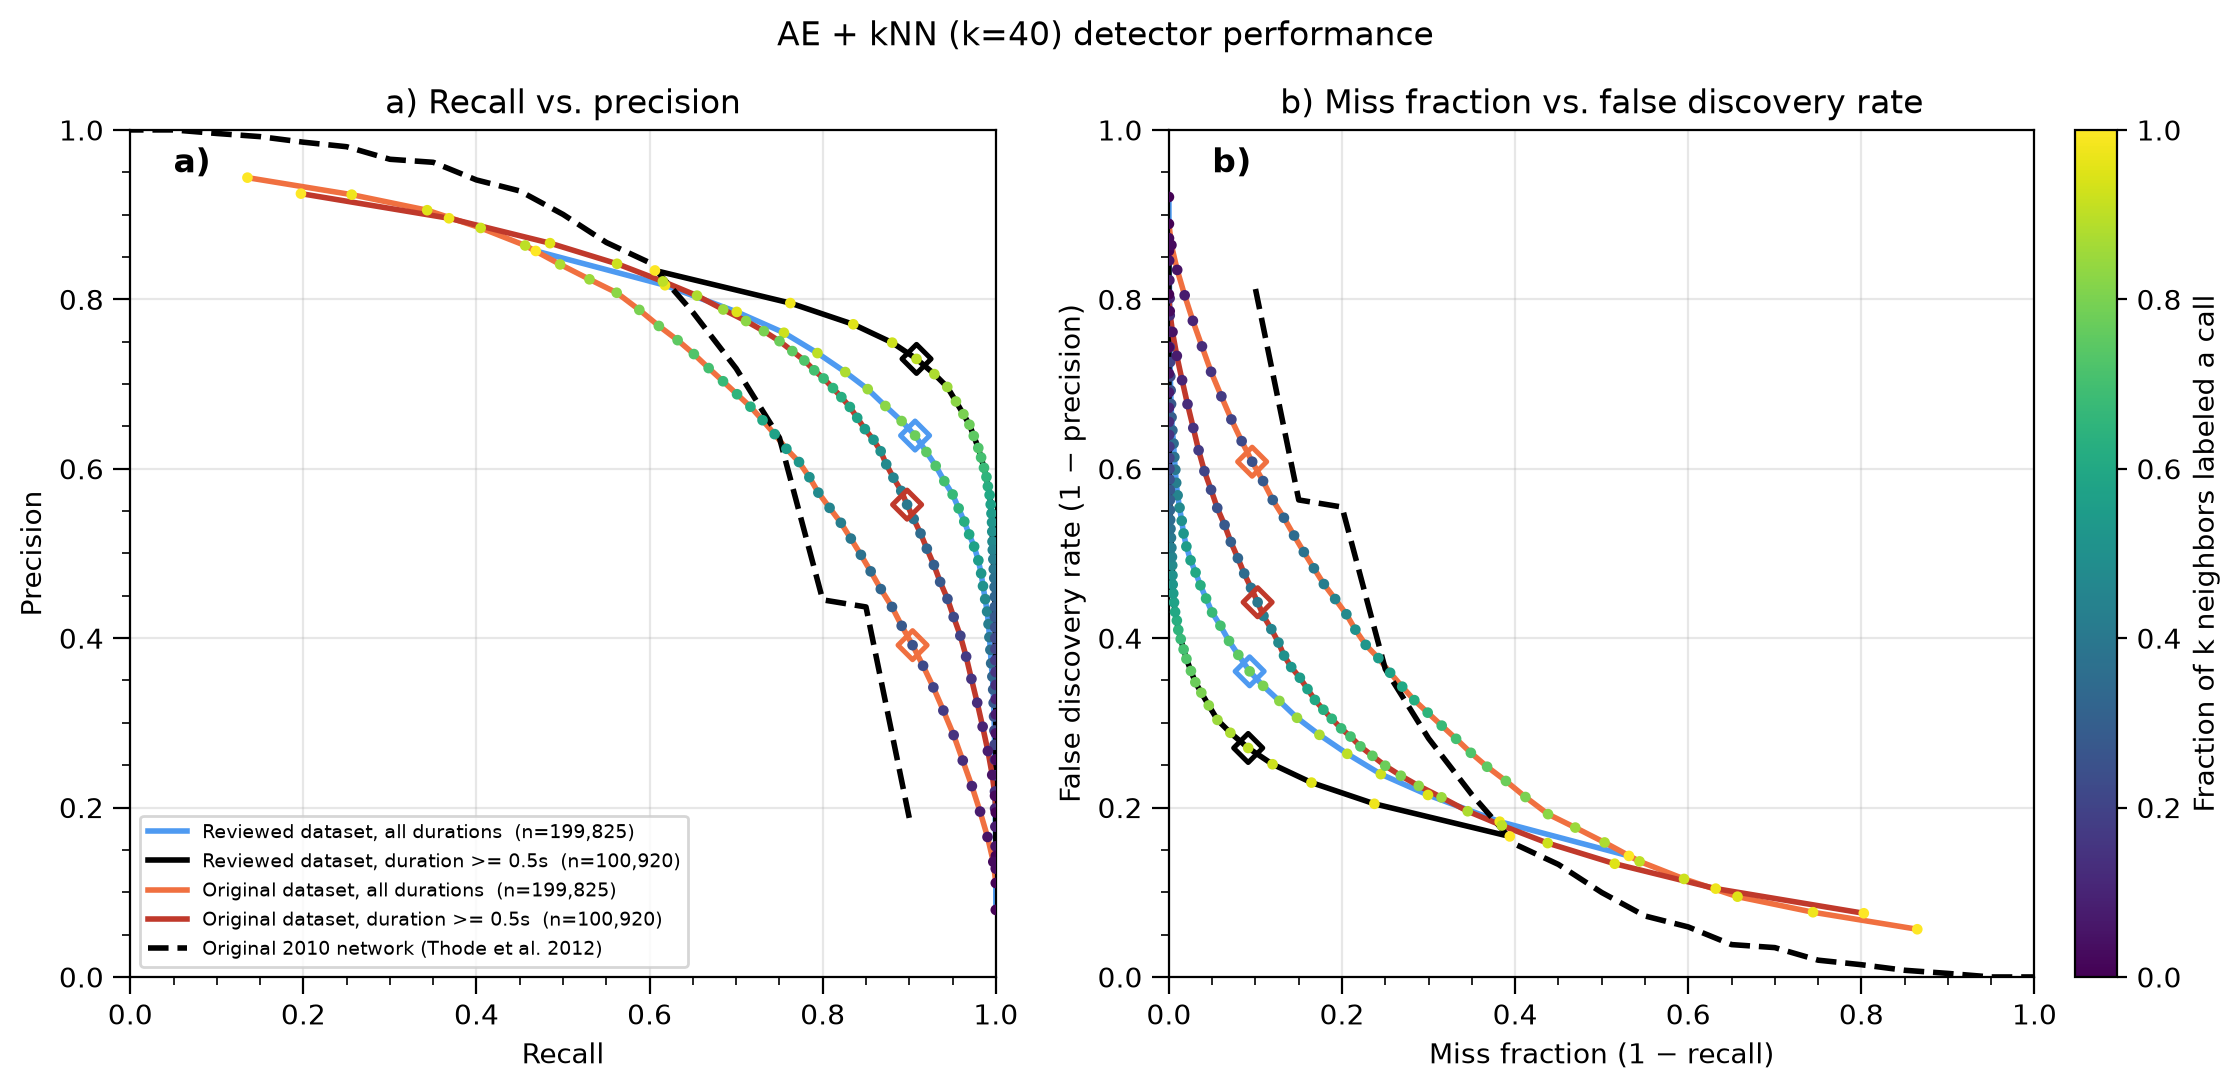
\includegraphics[width=1\linewidth]{Figures/ae_knn_miss_vs_fdr.png}
    \caption{AE+kNN ($k$=40 neighbors) detector performance on the 199,825-spectrogram independent evaluation set, as the neighbor-vote threshold (fraction of $k$ nearest training neighbors labeled a call; colorbar) is swept. a) Recall vs.\ precision. b) Miss fraction vs.\ false discovery rate. Blue/black: reviewed (post-UMAP) labels, without and with a $\geq$0.5~s minimum call-duration filter, respectively; orange/red: original (pre-UMAP) labels, without and with the same duration filter. Black dashed line: the original 2010 detector \citep{thode2012automated}, combined across the four field seasons (2008, 2010, 2012, 2014) weighted by each season's sample count. Diamond markers indicate the matched miss-fraction=10\% operating point reported in Table~\ref{tab:ae_knn_results}.}
    \label{fig:AE_result}
\end{figure}

**Table~\ref{tab:ae_knn_results} summarizes this same neighbor-vote detector at a
matched operating point of miss fraction = 10\% ($k$=40 neighbors) for every
label-set/duration-filter combination in this study, alongside the natural,
unfiltered ``accept every candidate'' baseline for each label set. Fixing
the miss fraction (rather than the vote threshold) puts every row at the
same recall level, so the raw-vs-reviewed and duration-filter comparisons
isolate the effect of the dataset review and the duration filter,
respectively, from any confound of the four conditions otherwise landing at
different recall levels. Because this detector requires no training beyond the unsupervised
autoencoder itself and only a single hyperparameter (the neighbor-vote
threshold), it is currently our most readily reproducible detection result, and
we recommend it as the primary point of comparison against the original 2010
detector \cite{thode2012automated}.**

\begin{table}[ht]
    \centering
    \caption{**AE+kNN nearest-neighbor detector performance on the
    199,825-spectrogram independent evaluation set ($k$=40 neighbors),
    comparing the original (pre-UMAP) vs.\ manually reviewed (post-UMAP)
    label sets, with and without a minimum call-duration filter, and against
    each label set's own natural, unfiltered baseline.** Column definitions --
    \emph{Label set}: original (pre-UMAP, \texttt{type\_org}$>$0) vs.\
    manually reviewed (post-UMAP, \texttt{iscall}) annotation version
    (Sec.~\ref{sec:DatasetEditing}). \emph{Duration filter}: minimum call
    duration applied to evaluation transients before scoring (\emph{n/a} for
    baseline rows, which accept every candidate transient as a call, so no
    filter applies). \emph{Vote threshold}: fraction of the $k$=40 nearest
    training-set latent neighbors labeled a call required to flag a sample as
    a call; set per row to hit the matched miss fraction below (\emph{n/a}
    for baseline rows). \emph{Miss fraction}: $1-$recall (fixed at
    $\approx$10\% for the four detector rows; exactly 0\% for the baseline
    rows by construction). \emph{FDR}: false discovery rate, $1-$precision.
    \emph{FP:TP}: false positives per true call at that operating point, in
    the same units as the original 2010 detector's own natural, unfiltered
    ``roughly 8:1'' baseline (Ref.~\citenum{thode2012automated}; consistent
    with the 8.02:1 value recovered here for the original-label baseline
    row).}
    \label{tab:ae_knn_results}
    \begin{tabular}{|l|c|c|c|c|c|}
        \hline
        Label set & Duration filter & Vote threshold & Miss fraction & FDR & FP:TP \\
        \hline
        Reviewed (post-UMAP) & n/a (accept all)  & n/a   & 0.0\%  & 0.921 & 11.64 \\
        Original (pre-UMAP)  & n/a (accept all)  & n/a   & 0.0\%  & 0.889 & 8.02 \\
        \hline
        Reviewed (post-UMAP) & all durations     & 0.775 & 9.3\%  & 0.361 & 0.56 \\
        Reviewed (post-UMAP) & $\geq$0.5 s        & 0.900 & 9.2\%  & 0.270 & 0.37 \\
        Original (pre-UMAP)  & all durations     & 0.250 & 9.6\%  & 0.608 & 1.55 \\
        Original (pre-UMAP)  & $\geq$0.5 s        & 0.400 & 10.2\% & 0.442 & 0.79 \\
        \hline
    \end{tabular}
\end{table}

**At this matched $\approx$10\% miss fraction, the AE+kNN detector reduces the
false-positive-to-true-call ratio from the natural, unfiltered baseline (8.02
for original labels, 11.64 for reviewed labels -- both far worse than the
2010 detector's own reported $\sim$8:1, since the reviewed baseline reflects a
lower call prevalence than the original) down to between 0.37:1 and 1.55:1
depending on label set and duration filter -- roughly a 5- to 21-fold
reduction relative to each label set's own baseline. Holding the label set
fixed, the duration filter alone improves FP:TP substantially in both cases
(reviewed: 0.56$\to$0.37; original: 1.55$\to$0.79). Holding the duration
filter fixed, dataset review improves FP:TP by roughly a factor of 2--3
at this matched recall level (all durations: 1.55$\to$0.56; $\geq$0.5~s:
0.79$\to$0.37), directly isolating the review's effect on this detector from
any confound of the two label sets reaching the 10\% miss target at different
vote thresholds. The reviewed-label, duration-filtered
configuration offers the best operating point in this comparison
(FP:TP=0.37 at 9.2\% miss), while the original, unfiltered labels remain the
most directly comparable to the 2010 detector's own reported baseline
convention.**

% --- Superseded: this figure's content (miss vs. FDR curves) is now merged
% --- into Figure~\ref{fig:AE_result} above as panel b), alongside a matching
% --- recall-vs-precision panel a); kept here for reference.
% **\begin{figure}[htbp]
%     \centering
%     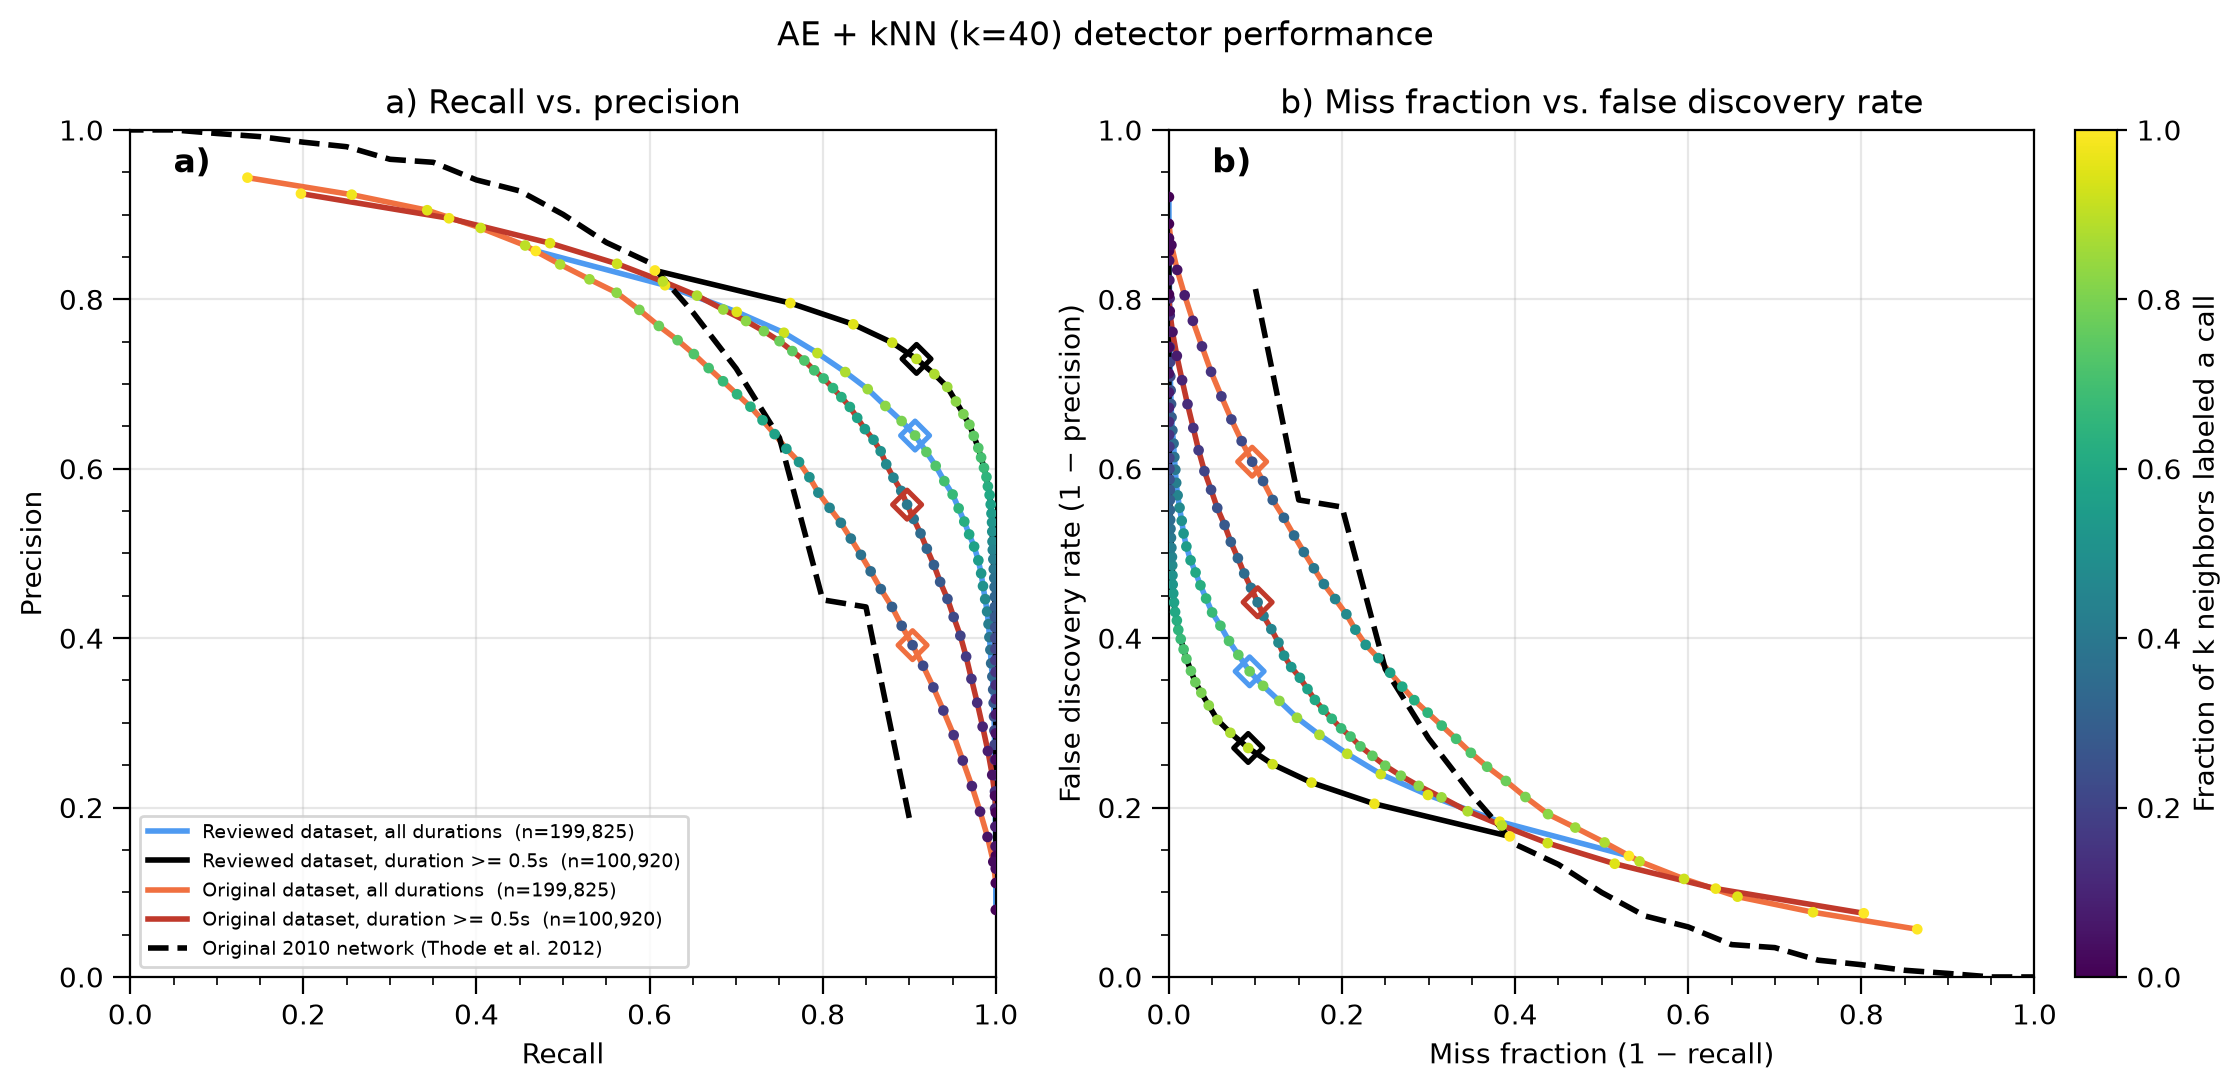
\includegraphics[width=0.85\linewidth]{Figures/ae_knn_miss_vs_fdr.png}
%     \caption{Miss fraction vs.\ false discovery rate for the AE+kNN detector
%     ($k$=40 neighbors) as the neighbor-vote threshold is swept, evaluated on the
%     199,825-spectrogram independent evaluation set under both the original and
%     manually-reviewed (post-UMAP) label sets, with and without a minimum call
%     duration of 0.5~s. The marked operating point (vote threshold=0.75)
%     corresponds to the values reported in Table~\ref{tab:ae_knn_results}.}
%     \label{fig:ae_knn_miss_vs_fdr}
% \end{figure}**

\subsection{Cold-start CNN vs.\ other CNN-family detectors}
\label{sec:CNNFamily}

Beyond the scratch-vs-warm-start comparison above, it is useful to place the
scratch ("cold-start") CNN in the context of other CNN-family detectors
evaluated in this study: the same warm-start CNN, a frozen pretrained
bioacoustic CNN (BirdNET/Perch 2.0) with a linear probe, and two frozen
general-purpose ImageNet CNN backbones (ResNet-18, EfficientNet-B0) with
linear probes. All figures below use the \emph{original}, pre-review label
set, since not every model in this comparison has been re-scored against the
manually reviewed labels of Sec.~\ref{sec:DatasetEditing}; the exact
evaluation protocol differs by model and is noted individually, so these
numbers should be read as a general orientation rather than a perfectly
controlled, single-protocol comparison (Table~\ref{tab:cnn_family_summary}).

\begin{table}[ht]
    \centering
    \caption{Cold-start CNN vs.\ other CNN-family detectors, original
    (pre-review) labels. Protocols differ by model (see notes); this is an
    orientation comparison, not a single controlled experiment.}
    \label{tab:cnn_family_summary}
    \begin{tabular}{|l|c|c|c|l|}
        \hline
        Model & $N$ & AP & ROC-AUC & Protocol \\
        \hline
        Scratch CNN (cold start)   & 199{,}825 & 0.809 & 0.964 & Full independent eval set \\
        Warm-start CNN (AE-init)   & 199{,}825 & 0.787 & 0.956 & Full independent eval set \\
        BirdNET/Perch 2.0          & 4{,}000   & 0.483 & 0.803 & Subsample, Griffin-Lim + linear probe \\
        ResNet-18 (ImageNet)       & 199{,}825 & 0.664 & 0.889 & Grouped 15\% held-out split, linear probe \\
        EfficientNet-B0 (ImageNet) & 199{,}825 & 0.713 & 0.913 & Grouped 15\% held-out split, linear probe \\
        \hline
    \end{tabular}
\end{table}

\begin{figure}[htbp]
    \centering
    \includegraphics[width=0.9\linewidth]{Figures/cnn_family_summary_bars.png}
    \caption{Average precision and ROC-AUC for the cold-start (scratch) CNN
    (red) versus the other CNN-family detectors evaluated in this study
    (blue), original labels. See Table~\ref{tab:cnn_family_summary} for exact
    $N$ and evaluation protocol per model.}
    \label{fig:cnn_family_summary_bars}
\end{figure}

Full precision-recall / FDR-vs-miss curves are reproducible in this study for
three of the five models -- scratch CNN, warm-start CNN, and BirdNET/Perch
2.0 -- whose per-threshold arrays were saved end-to-end; they are shown as
separate, single-model figures below rather than overlaid, since they are not
all scored under an identical protocol (full eval set for the two custom
CNNs vs.\ a 4,000-image subsample for BirdNET/Perch 2.0).

\begin{figure}[htbp]
    \centering
    \includegraphics[width=1\linewidth]{Figures/cnn_coldstart_pr_fdr.png}
    \caption{Scratch CNN (cold start), precision-recall and FDR-vs-miss-fraction
    curves on the full 199,825-spectrogram independent evaluation set,
    original labels (AP=0.809, ROC-AUC=0.964).}
    \label{fig:cnn_coldstart_pr_fdr}
\end{figure}

\begin{figure}[htbp]
    \centering
    \includegraphics[width=1\linewidth]{Figures/warmstart_cnn_pr_fdr.png}
    \caption{Warm-start CNN (AE-initialized), precision-recall and
    FDR-vs-miss-fraction curves on the full 199,825-spectrogram independent
    evaluation set, original labels (AP=0.787, ROC-AUC=0.956).}
    \label{fig:warmstart_cnn_pr_fdr}
\end{figure}

\begin{figure}[htbp]
    \centering
    \includegraphics[width=1\linewidth]{Figures/birdnet_perch_pr_fdr.png}
    \caption{BirdNET/Perch 2.0 (frozen pretrained bioacoustic CNN + linear
    probe), precision-recall and FDR-vs-miss-fraction curves on a 4,000-image
    subsample of the independent evaluation set, original labels (AP=0.483,
    ROC-AUC=0.803).}
    \label{fig:birdnet_perch_pr_fdr}
\end{figure}

At the level of scalar summary metrics (Table~\ref{tab:cnn_family_summary},
Fig.~\ref{fig:cnn_family_summary_bars}), the cold-start CNN is the strongest
detector in this comparison on both AP and ROC-AUC, ahead of the warm-start
CNN by a narrow margin (as already noted above) and ahead of every frozen,
non-task-trained backbone by a substantially larger margin: +0.10--0.33 AP
and +0.05--0.16 ROC-AUC over BirdNET/Perch 2.0, ResNet-18, and
EfficientNet-B0. This is consistent with the expectation that a classifier
trained end-to-end on this task's own spectrogram distribution outperforms
frozen embeddings from backbones pretrained on a different domain (natural
images, for ResNet-18/EfficientNet-B0) or a related-but-distinct bioacoustic
task (BirdNET/Perch 2.0), even when the latter are paired with a
task-specific linear probe. We caution that this is not a strictly controlled
comparison: the two ImageNet-backbone rows (ResNet-18, EfficientNet-B0) were
scored under a different protocol (grouped 15\% held-out split of the eval
directory) than the two custom CNNs (full 199,825-image independent
evaluation) and BirdNET/Perch 2.0 (a 4,000-image subsample with Griffin-Lim
spectrogram reconstruction), and an AST-style ViT backbone from the same
benchmark family was not available in this evaluation pass. A fully
protocol-matched re-evaluation of the two ImageNet backbones on the identical
full evaluation set would be needed to sharpen those two rows into a fully
rigorous ranking alongside the other three models, whose curves are already
reproduced on either the full evaluation set or a fixed subsample above.


\section{Discussion}

% -the value of using latent space for reviewing user errors

% -sensitivity to time window.
\subsection{The value of the latent space for reviewing dataset and labeling errors}

Beyond serving as a feature-extraction backbone for the supervised classifier
(Sec.~\ref{sec:cnn_classifier}), the autoencoder's 32-dimensional latent space
proved useful as a diagnostic tool for auditing the training dataset itself.
Because every spectrogram in the 100,000-image pool has a corresponding point
in this compressed representation, the full dataset could be visualized as a
low-dimensional UMAP projection (Sec.~\ref{sec:autoencoder}) and inspected by
neighborhood rather than by exhaustively re-listening to or re-viewing
spectrograms in collection order. This was the practical mechanism behind the
dataset-editing pass described in Sec.~\ref{sec:DatasetEditing}: images
containing multiple overlapping signals, whale calls that had not been logged
in the manual database, and transients that had been mislabeled as calls
(most often airgun pulses masking a genuine call) were located by identifying
anomalous or mixed-label clusters in the latent-space projection and then
auditing the comparatively small number of spectrograms responsible for them,
rather than by reviewing the entire corpus. In effect, the latent space turns
the problem of finding labeling errors scattered across tens of thousands of
automatically-compiled images into the much smaller problem of explaining a
handful of outlying or mixed clusters — an approach whose value should only
grow as automatically-labeled bioacoustic datasets reach a scale (Sec.~\ref{sec:1})
that precludes full manual re-verification. We note that this account of the
latent space's diagnostic value is qualitative: we did not separately track
how many labeling corrections were made through this route versus other QA
steps, nor compare it against alternative auditing strategies (e.g., ranking
by classifier confidence or reconstruction error alone); quantifying the
efficiency of latent-space-guided auditing relative to these alternatives
would be a natural follow-up analysis.

\subsection{Sensitivity to time-window alignment}

A design choice with implications for both the autoencoder and the
downstream classifier is the fixed-duration, peak-power-centered spectrogram
window described in Sec.~\ref{sec:EventDetection}: rather than aligning each
image to, for example, the detector's onset time, every spectrogram is
centered on the time of maximum local power spectral density encountered
between 25 and 450 Hz. This choice was made specifically to reduce the
tendency of the autoencoder to encode a signal's absolute temporal position
within the window as a latent feature, since a purely reconstructive
objective has no explicit incentive toward time-shift invariance and would
otherwise be free to map same-call, different-alignment spectrograms to
different, disconnected regions of the latent space.

We have not, however, performed a controlled ablation that directly
quantifies how sensitive either the latent representation or the downstream
classifier's accuracy is to this alignment convention — for example, by
re-centering the same held-out calls at several offsets from the peak-power
point and measuring the resulting change in embedding distance or classifier
score. The consistency of classifier performance across four field seasons,
two DASAR sites, and three DASAR channels (Sec.~\ref{sec:Results}) is
reassuring but only an indirect argument, since it does not rule out the
alignment convention behaving differently for calls of different type,
duration, or SNR than it does in aggregate. We therefore flag this
explicitly as an open question rather than a validated property of the
pipeline: a direct sensitivity analysis along these lines would clarify
whether peak-power centering is a genuine robustness safeguard, a
performance-neutral convention, or a source of latent hidden bias inherited
from the original detection pipeline (Sec.~\ref{sec:EventDetection}).

\section{\label{sec:Conclusion}Conclusion}

We built and evaluated a two-stage deep learning pipeline — an unsupervised
convolutional autoencoder followed by a supervised convolutional classifier
sharing its encoder architecture — for distinguishing bowhead whale calls
from other transient sounds, including seismic airgun pulses, in passive
acoustic recordings from the Alaskan North Slope. Both a randomly-initialized
classifier and a classifier warm-started from the autoencoder's encoder
weights were trained on an identical, leakage-controlled 100,000-sample
dataset and evaluated, without further tuning, on a fully independent
held-out set of 199,825 spectrograms spanning four field seasons (2008,
2010, 2012, 2014), two DASAR sites, and three DASAR channels
(Table~\ref{tab:benchmark_results}). Both classifiers generalized well and
similarly to this unseen data (ROC-AUC of 0.959 and 0.956, average precision
of 0.805 and 0.787, for the scratch and warm-start models respectively), and
this small performance gap was stable across every year/site/DASAR subgroup
examined (Sec.~\ref{sec:Results}), indicating a genuine, if modest, property
of the two initialization strategies on this task rather than an artifact of
a particular subset of the data. Contrary to our initial expectation,
unsupervised autoencoder pretraining did not confer a measurable
generalization advantage over training the same architecture from random
initialization on this dataset. **A simpler nearest-neighbor detector built
directly on the autoencoder's 32-dimensional latent space, requiring no
supervised training at all, reduced the false-positive-to-true-call ratio,
at a matched 10\% miss-fraction operating point, from each label set's own
natural, unfiltered baseline (8.02:1 original, 11.64:1 reviewed) to between
0.37:1 and 1.55:1 depending on label set and duration filter
(Sec.~\ref{sec:AEkNN}, Table~\ref{tab:ae_knn_results}); because it depends on
only a single hyperparameter, this AE+kNN result is currently our most
readily reproducible finding and the one we recommend as the primary point
of comparison against the original 2010 detector.**

Two aspects of the pipeline merit further attention, as discussed above.
First, the autoencoder's latent space proved to be a practical tool for
auditing the training dataset for labeling errors (Sec.~\ref{sec:DatasetEditing}),
suggesting that latent-space-guided review could be formalized into a
reusable quality-assurance step for future automatically-compiled bioacoustic
datasets, rather than remaining an ad hoc part of dataset construction.
Second, while the spectrogram images are deliberately centered on peak local
power to reduce time-shift sensitivity in the latent space, we have not
directly measured how sensitive detection performance or the latent
representation itself is to this alignment convention, and we flag this as a
concrete direction for follow-up analysis. More broadly, this detector
operates at the coarse level of distinguishing a call from a non-call
transient; the seven manually-annotated call sub-types (Types 1--7) present
in the training data were not modeled here, and discriminating among them
remains an open target for future work building on the representation
developed in this study. A companion probing study (in preparation)
finds that call-sub-type information is linearly decodable from these same
embeddings well above chance, but is not recovered by standard unsupervised
clustering, suggesting that the linear frequency axis used throughout this
work may disperse harmonic sub-type structure (Sec.~\ref{sec:1}) across
several entangled latent dimensions rather than concentrating it along an
axis a clustering algorithm can exploit. A natural next step is therefore to
warp each spectrogram's frequency axis onto a logarithmic, constant-$Q$ grid
before the encoder \citep{brown1991calculation} -- so that a stack of $N$
harmonics of a fundamental $F_0$ occupies the same pixel spacing regardless
of $F_0$ -- and to compare this representation against pitch-aware
convolutional architectures developed for a similar purpose in music and
speech processing \citep{kim2018crepe}.


\begin{acknowledgments}
This research was supported by  North Pacific Research Board as Project F2410. 
\end{acknowledgments}




% \section{Making the Bibliography Using BibTeX}
% Authors are highly  recommended to use BibTeX to produce their
% bibliographies. The results will be predictable and even if
% it might take some time to get comfortable with  using BibTeX,
% in the long run it will save you endless aggravation.

% A resource for making your bibliography entries
% correctly is included in this package: 
% JASA-ReferenceStyles.pdf. You will also find
% the files
% bibsamp1.tex/.pdf and bibsamp2.tex/.pdf
% for examples of output; and sampbib.bib for an example of
% how to make your .bib database entries.

% There are two possible bibliography styles: the default, author-year,
% and the optional style, Numbered\-Refs, which you would call using\\
% {\verb+\documentclass[preprint,NumberedRefs]{JASAnew}+ }

% Every \verb+\cite+ will produce a citation and an entry in the
% bibliography and every cite must have a matching entry in the bib
% database file.

% \verb+\citep{}+ should be used rather than \verb+\cite{}+
% Note that the citations are hyperlinked to their entries in the
% bibliography:

% Normal journal cite: \citep{joursamp1},
%  Book reference \citep{booksamp1},
% In press, \citep{inpress3}. 
% Computer language documentation:
% \citep{sampcode2}.


% \begin{quote}
% \it
% NOTE:\\
% Once you have used BibTeX you
% should open the resulting .bbl file and cut and paste the entire contents 
% into the end of your article. You should also comment out
% \verb+\bibliography{<your .bib file>}+, ie,
% \verb+%\bibliography{<your .bib file>}+.
% \end{quote}

% Make your bibliography by doing: pdflatex filename,  bibtex filename,
% pdflatex filename, pdflatex filename.

% {\bfseries\itshape
% Compare the results you get with\\
% {\verb+\documentclass[preprint]{JASAnew}+ }\\
% vs.\\
% {\verb+\documentclass[preprint,NumberedRefs]{JASAnew}+ }
% }

\bibliography{Bowhead_AI_references.bib}


\end{document}
